\subsubsection{Diseño de estructura}
Tomando en consideración todos los sistemas que estarán montados, así como las piezas, fijas y estáticas, se diseñó la siguiente estructura
 (Figura \ref{fg:Estructura}). 

\begin{figure}[h]
    \centering
        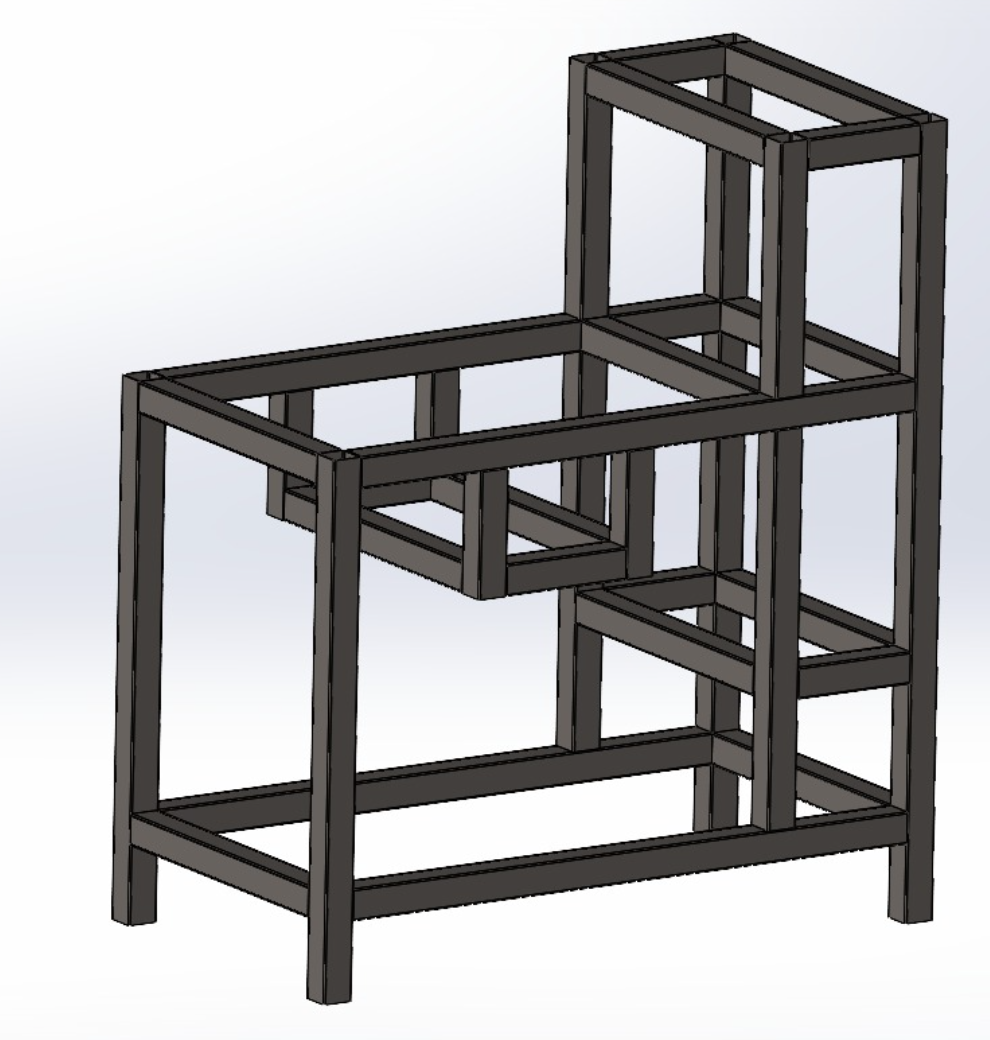
\includegraphics[scale=0.6]{images/Capitulo 4/S6/Estructura.png}
        \caption{Estructura}
    \label{fg:Estructura}
\end{figure}

La estructura cuenta con un soporte horizontal del lado derecho, sobre el cual será montado el motor encargado de generar el torque necesario para poner en rotación al eje interno de la cámara de agitación, el espacio que se encuentra entre ese soporte y el extremo derecho de la estructura es el espacio confinado para el movimiento de la banda tipo 3V encargada de transmitir esa fuerza de rotación.

En la parte superior derecha de la imagen (Figura \ref{fg:Estructura}), será ubicado el sistema de trituración y en el espacio frontal se instalará el sistema de control de todo el compostador.

Se utilizo un perfil PTR 2x2 C14 para tener el suficiente ancho para montar y atornillar los componentes, así como para tener una estructura lo suficientemente rígida y sin deformaciones que afectaran la rotación normal del eje del compostador.

Esta estructura fue rediseñada en varias ocasiones hasta llegar a la estructura actual, en la cual se tiene en consideración todos y cada uno de los sistemas que se implementarán para su correcto funcionamiento.







